\documentclass[10pt]{article}
\usepackage[pdftex]{graphicx}
\graphicspath{{./images/}}
\usepackage{amsmath,amssymb}
\usepackage{dirtytalk}
\usepackage{anyfontsize}
\usepackage{xcolor}
\usepackage{hyperref}
\hypersetup{
	colorlinks,
	linkcolor={red!50!black},
	citecolor={blue!50!black},
	urlcolor={blue!80!black}
}
\usepackage[skip=10pt plus1pt, indent=40pt]{parskip}
\usepackage{../../common_styles/csagh}


\begin{document}
	\begin{opening}
		\title{Entregable 1 - PIA}
		\author[Universidad Autónoma de Nuevo León, San Nicolás de los Garza, aldo.hernandezt@uanl.edu.mx]{Aldo Hernández}
		\author[Universidad Autónoma de Nuevo León, San Nicolás de los Garza, abraham.lopezg@uanl.edu.mx]{Abraham López}
		\author[Universidad Autónoma de Nuevo León, San Nicolás de los Garza, gilberto.garciam@uanl.edu.mx]{Damián García}
		\author[Universidad Autónoma de Nuevo León, San Nicolás de los Garza, cristian.antoniosnt@uanl.edu.mx]{Cristian Antonio}
		
		\keywords{...}
		\begin{abstract}
			En este documento seleccionamos nuestro conjunto de datos (imágenes) para realizar nuestro proyecto integrador de aprendizaje. Este proyecto tendrá la finalidad de crear una red neuronal artificial que clasifique las letras de palabras escritas a mano para su digitalización. El conjunto contiene un total de 413,701 registros divididos en tres subconjuntos: entrenamiento, prueba y validación, estos datos provienen de niños que escribieron a mano su nombre y apellido (si aplica) en algún papel. Finalmente, se detalla el cronograma con las distintas etapas del trabajo mediante un diagrama de Gantt según las fechas de entrega de cada documento semanal.
		\end{abstract}
		
		\keywords{python, dataset, exploración, análisis, pandas}
	\end{opening}
	
	\section{Selección del dataset}
	Para seleccionar nuestro conjunto de datos investigamos diferentes fuentes de información confiables. Comenzamos buscando información gubernamental de México en relación a la salud, concretamente acerca de dengue y COVID-19; sin embargo, descartamos estos conjuntos de datos debido a la poca (o casi nula) aplicación real debido a la cantidad de datos y columnas ya que tenían poco que ver con la predicción de un posible diagnóstico para dichas enfermedades. \par
	Posteriormente, encontramos en la plataforma \href{www.kaggle.com}{Kaggle} una serie de \textit{datasets} interesantes, pero finalmente nos decantamos por un conjunto de datos que contiene más de 400,000 transcripciones de nombres escritos por niños. \par
	Este \textit{dataset} es adecuado para una tarea de aprendizaje supervisado ya que contiene un gran número de imágenes etiquetadas para llevar a cabo una tarea de reconocimiento óptico de caracteres (Optical Character Recognition, OCR), además, estas imágenes tienen buena calidad y no tienen ruido visual. Por otra parte, podrían haber algunos detalles ya que al tratarse de nombres, podría haber un desbalanceo de clases para ciertas letras no tan comunes en nombres de personas, como podrían ser las letras x, y, z, q o w. También, al ser un conjunto de datos hecho en idioma inglés, no existe ningún registro con la letra ñ. Además, todos los nombres están en mayúsculas y a pesar de que algunos tienen tildes, estas no serán tomadas en cuenta. \par
	Fuera de esos detalles, consideramos que no hay ninguna otra complicación en relación al conjunto de datos, ya que solo se cuenta con dos columnas: la ruta hacia la imagen y el nombre asociado (en mayúsculas), y como a cada imagen le corresponde un nombre pues no hay problemas de datos faltantes. \par
	Finalmente, es importante mencionar que este \textit{dataset} ya está dividido en tres conjuntos importantes para el desarrollo de la red neuronal: entrenamiento, prueba y validación, así que en etapas posteriores ya no nos tendremos que preocupar en volverlas a separar.
	
	\section{Definición del problema}
	Al momento de escribir a mano notas o apuntes puede resultar complicado para el lector interpretar algunas letras o palabras, incluso si es "letra propia". Esto se debe a la infinidad de estilos y variantes que el ser humano puede presentar al escribir a mano, haciendo la tarea de reconocimiento de caracteres complicada tanto para una computadora como en ciertos casos a un ser humano. Es por esto que nos decidimos por este conjunto de datos, ya que queremos crear un modelo capaz de combatir dicha problemática. \par
	Es decir, buscamos reconocer palabras en imágenes escaneadas con texto escrito a mano para digitalizarlo mediante la clasificación de los caracteres según las diferentes maneras de escribir las letras del abecedario inglés.
	
	\section{Código inicial}
	Para el \textit{script} inicial usaremos la librería Pandas para la carga y exploración inicial de los datos. \par
	\begin{figure}[h]
		\centering
		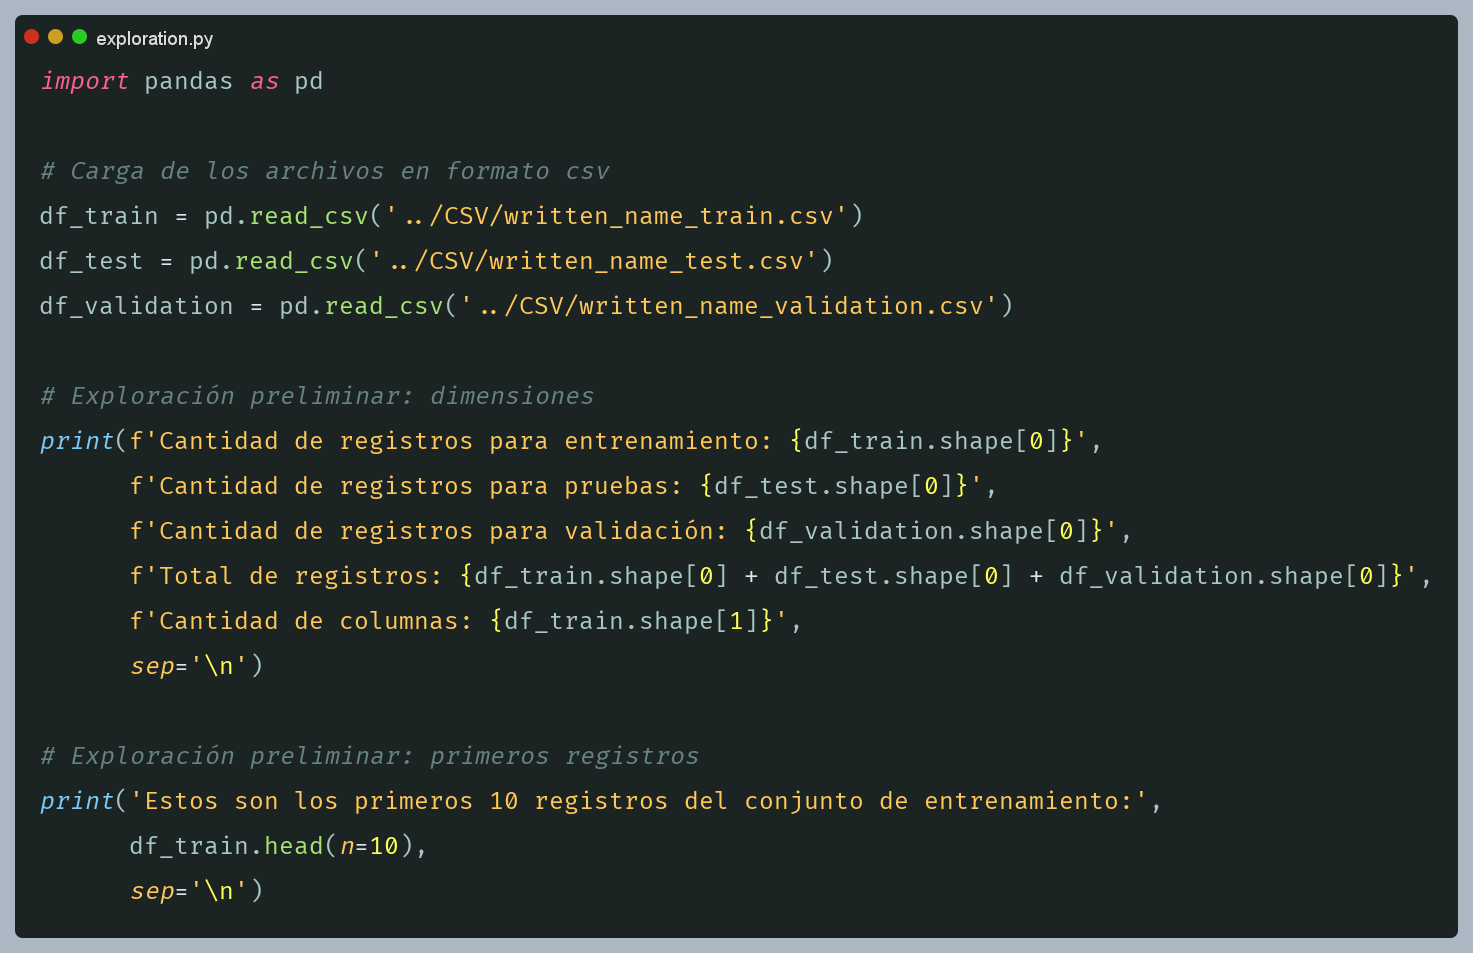
\includegraphics[width=120mm]{./images/script-inicial.jpg}
		\caption{Script inicial completo.}
	\end{figure}
	Como se puede observar, primero realizamos la carga de los tres \textit{datasets} que conforman el \textit{dataset} original: entrenamiento, prueba y validación. Seguido de ello investigamos las dimensiones de cada conjunto, como todos tendrán 2 columnas puesto que parten del mismo conjunto, solo nos centraremos en la cantidad de registros:
	\begin{itemize}
		\item Entrenamiento: 330,961 registros
		\item Prueba: 41,370 registros
		\item Validación: 41,370 registros
		\item Total: 413,701 registros
	\end{itemize}
	
	\newpage
	Además, podemos ver los primeros 10 registros del conjunto de entrenamiento en la siguiente tabla: \par
	\begin{table}[!ht]
		\centering
		\caption{Primeros registros de entrenamiento}
		\begin{tabular}{|c|c|c|}
			\hline
			\# & FILENAME & IDENTITY \\
			\hline
			0 & TRAIN\_00001.jpg & BALTHAZAR \\
			\hline
			1 & TRAIN\_00002.jpg & SIMON \\
			\hline
			2 & TRAIN\_00003.jpg & BENES \\
			\hline
			3 & TRAIN\_00004.jpg & LA LOVE \\
			\hline
			4 & TRAIN\_00005.jpg & DAPHNE \\
			\hline
			5 & TRAIN\_00006.jpg & LUCIE \\
			\hline
			6 & TRAIN\_00007.jpg & NASSIM \\
			\hline
			7 & TRAIN\_00008.jpg & ASSRAOUI \\
			\hline
			8 & TRAIN\_00009.jpg & LAVIAN \\
			\hline
			9 & TRAIN\_00010.jpg & MAEVA \\
			\hline
		\end{tabular}
	\end{table}
	Viendo estos primeros datos, nos damos cuenta de que la columna "IDENTITY" es la que contiene las etiquetas con los nombres y apellidos de todos los niños, con su respectivo archivo correspondiente.
	
	\section{Planificación}
	Para el diseño de nuestro cronograma, decidimos utilizar un diagrama de Gantt que va desde el día posterior a la fecha de entrega de este documento hasta el día anterior a la finalización del semestre. \par
	\begin{figure}[!h]
		\centering
		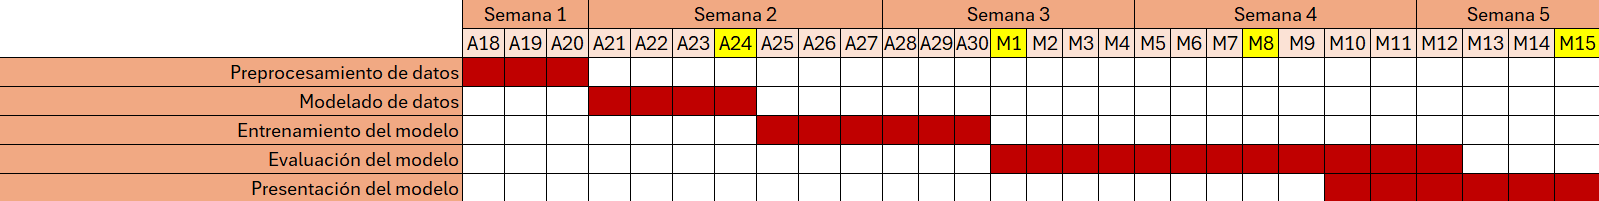
\includegraphics[width=120mm]{./images/cronograma.png}
		\caption{Diagrama de Gantt para la realización del PIA.}
	\end{figure}
	Estas principales etapas del proyecto serán realizadas de forma que todos los integrantes colaboremos activamente en cada una de ellas, supervisando cada aspecto antes de hacer la entrega del documento correspondiente. \par 
	La mayoría de las fases (en el mejor de los casos) no pueden llevarse a cabo al mismo tiempo debido a que cada una depende de la anterior, por ejemplo la evaluación requiere un buen entrenamiento, que a su vez necesita un modelado de los datos que tiene que ser llevado a cabo después de preprocesar la información; sin embargo, la presentación del proyecto es una excepción porque conlleva la realización de otros materiales no relacionados directamente con el modelo, como gráficas, resultados y documentos de presentación finales. También, se puede notar que la etapa de evaluación del modelo toma unos cuantos días incluso después de la fecha del documento entregable para dicha etapa, esto es debido a que si al momento de llegar a la fecha de entrega no estamos satisfechos con los resultados del modelo, podríamos implementar cambios (por ejemplo en los hiperparámetros) con la finalidad de conseguir un mejor modelo para la fecha final de entrega del proyecto.
	
\end{document}